\documentclass[10pt]{article}

\usepackage{amsmath}
\usepackage{amssymb}
\usepackage{graphicx}

\counterwithin*{equation}{section}
\counterwithin*{equation}{subsection}

\graphicspath{ {./images/} } 

\begin{document}
\section{Vectors}
Vectors have a magnitude(length) and direction.\\
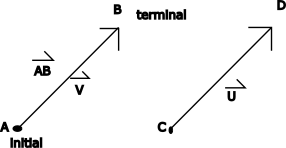
\includegraphics{somevectors}\\ $\vec{u}$ \& $\vec{v}$ have the same direction and magnitude, $\therefore$ they are equivalent.

\bigskip
\underline{Zero Vector} $\vec{O}$ has length zero. 

\bigskip
Vectors appear in forces, position, velocity, acceleration, torque, displacement, images.

\underline{Sums} $\vec{u}+\vec{v} = \vec{v}+\vec{u}$ 
 
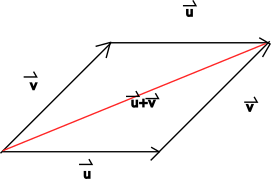
\includegraphics{sumvector} 
 
\underline{Scalar Multiplication}
\begin{itemize}
	\item If $c\in\mathbb{R}$, then vector $c \vec{v}$ has length |c| times the length of $\vec{v}$ and \begin{itemize} 
		\item the same direction as $\vec{v}$ if $c > 0$ 
		\item opposite direction as $\vec{v}$ if $c < 0$ 
	\end{itemize}
	\item If $c=0$ or $\vec{v} = \vec{o}$, then $c \vec{v} = 0$ 
\end{itemize}

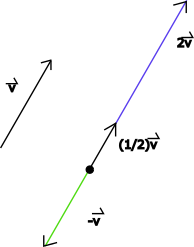
\includegraphics{scalarmult}

\underline{Differences} $\vec{u} - \vec{v} = \vec{u} + (-\vec{v})$ 

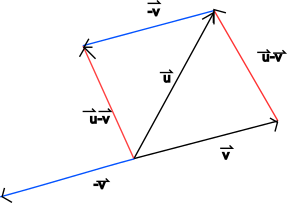
\includegraphics{vectordifference}

\underline{Ex:} Consider $\vec{u}\ and\ \vec{v}   $. Sketch $2 \vec{u}-\vec{v}$  

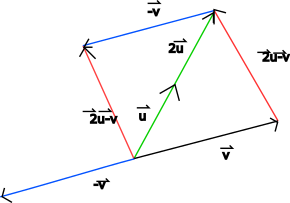
\includegraphics{vectordifference2}

\bigskip
\underline{Components}

\underline{2D:} $\vec{a} = <,a,b> $

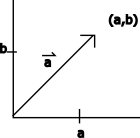
\includegraphics{vectorcomponents2d}

\underline{3D:} $\vec{a}=<a,b,c>  $

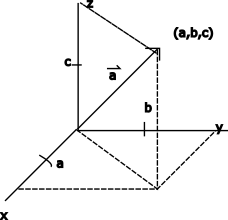
\includegraphics{vectorcomponents3d}

Sketch vectors equivalent to $\vec{a} = <2, -1>$ \\Choose any initial position in the graph. So long as it obeys the magnitude and direction of the vector it is valid.

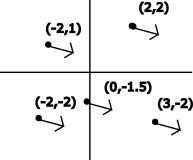
\includegraphics{equivalentvectors2d}

Unmarked in the graph is the point $o \vec{P}  $ which is the position vector for point $P$, otherwise known as the \underline{origin}.

Find components of the vector $\vec{a}  $ that has the following:\\\underline{Initial Point}: $(3,1)$\\\underline{Terminal Point}: $(-2,5)$

\bigskip
Vector $\vec{a}  $ has point $(-2-3,5-1)=(-5,4)$

Find components of the vector $\vec{b}  $ that has the following:\\\underline{Initial Point}: $(1,2,3)$\\\underline{Terminal Point}: $(-2,5,-7)$

\bigskip
Vector $\vec{a}  $ has point $(-2-1,5-2,-7-3)=(-3,3,-10)$

\bigskip
To sum up,
In general $\vec{AB}  $ has components $B(x_2,y_2),\ A(x_1,y_1) $ and is the result of $\vec{AB} =<x_2-x_1,y_2-y_1> $

\bigskip
Vector $\vec{ABC}  $ has components $B(x_2,y_2,z_2),\ A(x_1,y_1,z_1)$.\\It is the result of $\vec{ABC} =<x_2-x_1,y_2-y_1,z_2-z_1> $ 

\end{document}
